\documentclass[rnd]{mas_proposal}
% \documentclass[thesis]{mas_proposal}

\usepackage[utf8]{inputenc}
\usepackage{amsmath}
\usepackage{amsfonts}
\usepackage{amssymb}
\usepackage{graphicx}

\title{Evaluating Active Learning for 
Short Answer Grading}
\author{Mohandass Muthuraja, Jeeveeswaran Kishaan}
\supervisors{Prof. Paul G. Ploeger\\Deebul Nair }

% \thirdpartylogo{path/to/your/image}

\begin{document}

\maketitle

\pagestyle{plain}

\chapter{Introduction}
\begin{itemize}
    \item An introduction to the general topic you are covering.
    \item Why is it important? \\
\vspace*{1\baselineskip}

%Interactive short answer grading is a special case of automated short answer grading in which the learning algorithm is able to interactively query the human expert to obtain desired grades.
Short answer questions are characterized by the following aspects:

\begin{itemize}


\item the question must require a response that recalls external knowledge instead of requiring the answer to be recognized from within the question

\item the question must require a response given in natural language

\item the answer length should be roughly between one phrase and one paragraph

\item the assessment of the responses should focus on the content instead of writing style

\item the level of openness in open-ended versus close-ended responses should be restricted with an objective question design 

\end{itemize}

Automatic short answer grading essentially deals with using computational methods to predict the grades for the answers, thus cutting down the effort and time of teachers / professors. Many automated approaches have been proposed in the past for grading short answer questions. These methods compare how similar the students' answers are to the one provided by the teacher or professor and assign a grade proportional to the magnitude of similarity. Different approaches of computing these similarity measures include handcrafted pattern matching, automatic pattern matching, lexical similarity (how particular words effect other words), semantic similarity (deals with the meaning of sentences), and entailments (whether one sentence leads to another without any contradiction). The abovementioned methods all belong to a learning paradigm called supervised learning where the right answer for every question is available. Though these approaches were able to produce decent results, they suffer from many shortcomings such as;

\begin{itemize}

\item the failure to capture the different wordings/phrasing of the students while trying to answer the short answer questions. It is obvious that anticipating all different ways of answering his questions is practically impossible for the professor. 

\item lack of sufficient amount of labeled training data in the domain to learn the models. Reasons include privacy, availability, and the quality of the correct answers. 

\item accounting for small deviations in the answers which might affect the whole meaning of the sentence (for ex. in mathematical terms, though each and every word of the student's answer allign with that of the professor, a small negation or inverse operation would change the whole meaning).

\item finding a way to understand the underlying concept of various students' answers and bagging the similar ones (or the right and wrong ones separately) is also a very tedious task. \\

\end{itemize}

This work proposes a method where a system tries to learn this task of measuring the correctness of each answer with the help of a human in the loop. Active learning seems to be the best choice for this task as it actively queries
the human expert to grade the answer where the training utility of grading that particular answer is high. The query should be effective such that the response from the human expert is informative as possible. By actively selecting the data samples to label, it reduces the need for a considerable amount of labeled training samples thereby alleviating the problem of insufficient labeled data which is prevalent in supervised learning approaches.Thus, it tries to reduce the human effort of going through all the answers while improving it's understanding of the problem on a iterative basis. \\

The challenging task involved in following this approach is the selection of samples for which the labels could be queried from the human expert. Various active learning strategies are available to deal with the above mentioned challenge like querying on grading the most uncertain answers, answers that could increase the efficiency of grading system,answers that could reduce the generalization error etc.,


\end{itemize}





\section{Problem Statement}
\begin{itemize}
    \item What are you going to solve?
    \item How are you evaluating?
    
\vspace*{1\baselineskip}
    \item One of the biggest challenge involved in supervised learning is the need for large labeled datasets. Generating a large data for short answer grading is also an obstacle. Many automatic short answer grading systems rely on supervised learning techniques. This, in turn, leads to high annotation cost of labeling the large training data. Also, the workload for labeling the data is more.
    \item As new data are generated on a regular basis, retraining the model for every new data also have a caveat of high computation cost.  Developing a generic model to overcome the deficit of retraining the model for every new answer can solve this issue.
    \item Short answer grading typically focuses on the content rather than the style of writing. Short answers written by students have a lot of lexical diversity. Active learning can be used to handle the lexical diversity by involving human in training the model.
\end{itemize}


\chapter{Related Work}
\begin{itemize}
    \item What have other people done?
    \item Why is it not sufficient?
\end{itemize}

\section{Section 1}
\section{Section 2}



\chapter{Project Plan}

\section{Work Packages}
The bare minimum will include the following packages:
\begin{enumerate}
    \item[WP1] Literature Search
    \item[WP2] Experiments
    \item[WP3] Project Report
\end{enumerate}
Keep in mind that depending on your project, you will probably need to add work packages that are more suited to your projects.

\section{Milestones}
\begin{enumerate}
    \item[M1] Literature search
    \item[M2] Experimental setup
    \item[M3] Experimental Analysis
    \item[M4] Report submission
\end{enumerate}

\section{Project Schedule}
Include a gantt chart here. It doesn't have to be detailed, but it should include the milestones you mentioned above.
Make sure to include the writing of your report throughout the whole project, not just at the end.

\begin{figure}[h!]
    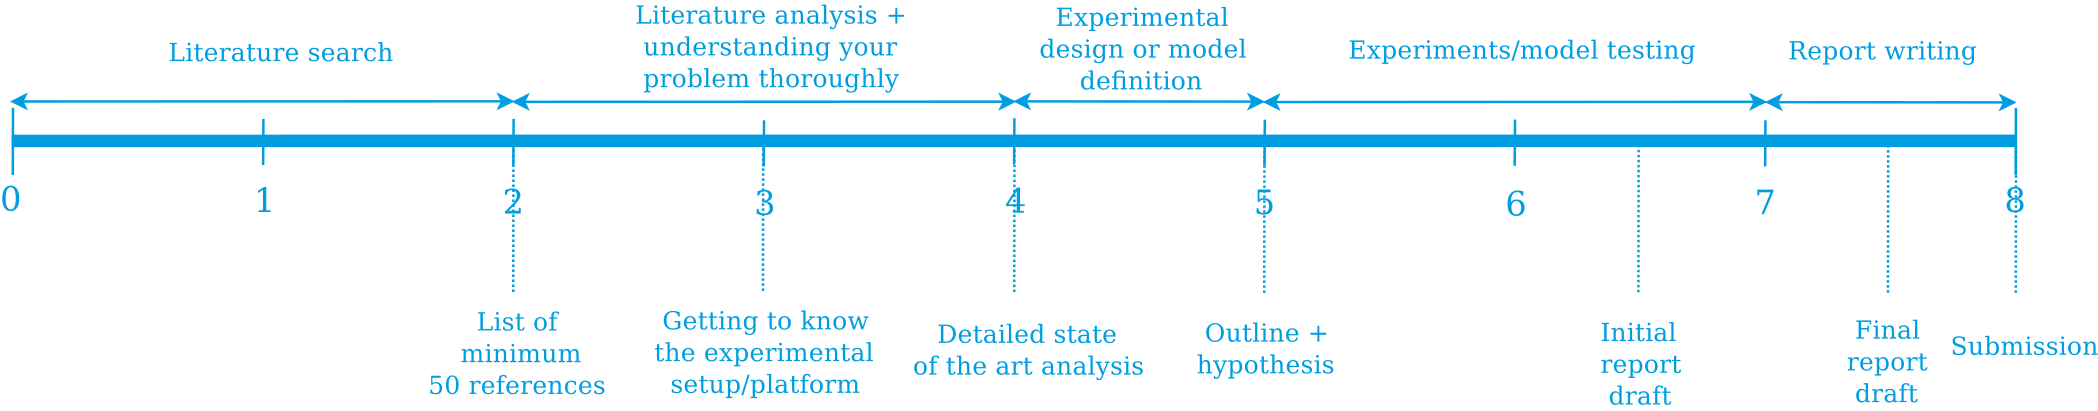
\includegraphics[width=\textwidth]{rnd_deliverable_timeline}
    \caption{}
    \label{}
\end{figure}

\section{Deliverables}
\subsection{Minimum Viable}

\begin{itemize}
    \item Survey the existing approaches for interactive short answer grading
    \item Review existing datasets for automatic short answer grading.
    \item Compile new datasets from different in-house domain
\end{itemize}

\subsection{Expected}
\begin{itemize}
    \item Evaluate the quality of different features for interactive short answer grading
    \item Evaluate Active Learning strategies for Short-Answer grading
    \item Implement a working model of 100 clicks for 1000 grades.
\end{itemize}

\subsection{Desired}
\begin{itemize}
    \item Integrate the best model with a graphical user interface(GUI)
\end{itemize}


\nocite{*}

\bibliographystyle{plainnat} % Use the plainnat bibliography style
\bibliography{bibliography.bib} % Use the bibliography.bib file as the source of references




\end{document}
